\documentclass[11pt]{article}
\usepackage[spanish]{babel}
\usepackage{natbib}  % Asegúrate de que esté esta línea
\bibliographystyle{apalike}  % Añade esto en el preámbulo
\usepackage[utf8]{inputenc}
\usepackage{amsmath}
\usepackage{graphicx}
\usepackage{natbib}
\usepackage{geometry}
\usepackage{booktabs}
\usepackage{hyperref}
\usepackage{caption}  % Añadir al preámbulo
\geometry{margin=2.5cm}
\setlength{\parindent}{0pt}
\title{Climatología de Estabilidad Atmosférica Marino-Costera con fines Eólicos}
\author{--}
%\date{\today}

\begin{document}

\maketitle

% ------------------------- INTRODUCCIÓN -------------------------
\section{Introducción}
La estabilidad atmosférica en la capa límite superficial es un factor necesario para optimizar la operación asociadas a actividades de energia eolica sobre oceano. Este informe presenta una metodología para estimar la frecuencia climatológica de condiciones \textbf{estables, inestables y neutras} mediante el cálculo de la longitud inversa de Obukhov (\(L_{inv}\)). Los resultados permiten identificar patrones horarios y mensuales en la región costera de Brasil (-21.6389°, -40.8693°) de interés. Los calculos y la logica de la estimacion se detallan en el github: https://github.com/Japq91/Obukhov/ 
% ------------------------- FUNDAMENTOS TEÓRICOS -------------------------
\section{Fundamentos Teóricos}
\subsection{Longitud de Obukhov en la Capa Límite}
Para el \citep{ecmwf_ifs_cy49r1_physics} la longitud de Obukhov ($L$) es un parámetro que caracteriza los efectos de flotabilidad en la turbulencia atmosférica cerca de la superficie. Se define como :

\begin{equation}
L = -\frac{u_*^3 \theta_v}{k g \overline{w'\theta_v'}}
\end{equation}

donde:
\begin{itemize}
    \item $u_*$: Velocidad de fricción (calculada en \texttt{obukhov\_calculate.py})
    \item $\theta_v$: Temperatura potencial virtual (derivada de \texttt{t2m} y \texttt{d2m} en ERA5)
    \item $\overline{w'\theta_v'}$: Flujo de calor sensible (variable \texttt{ishf} en ERA5)
    \item $k = 0.4$: Constante de von Kármán
\end{itemize}

\subsection{Interpretación Física}
Según \citep{ecmwf_obukhov_era5_guide}, los valores de $L$ determinan tres regímenes:
%

\begin{itemize}
    \item \textbf{Inestable} ($L < 0$): condiciones convectivas, flujo ascendente de calor desde la superficie. Favorece la turbulencia por flotabilidad. Dominada por convección (asociado a días soleados).
    
    \item \textbf{Estable} ($L > 0$): estratificación térmica estable, flujo descendente de calor. Inhibe la mezcla vertical. (asociado a noches despejadas).

    \item \textbf{Neutro} ($|L| \to \infty$): sin intercambio de calor sensible ($\overline{w'\theta'} \approx 0$), la turbulencia es generada solo por cizalladura.
\end{itemize}
%
\subsection{Implementación Numérica}

En el código, se calcula la longitud de Obukhov en su forma inversa ($L_{inv} = 1/L$) para evitar problemas numéricos con valores extremos (\(L \to \infty\)), normalizando dichos casos hacia cero:

\begin{equation}
L_{inv} = \frac{vk \cdot g \cdot tv_{*}}{tv_2 \cdot u_*^2}
\end{equation}

Esta ecuación corresponde a la línea 78 del script \texttt{obukhov\_calculate.py}, y se basa en las siguientes variables:

\begin{itemize}
    \item $vk$: Constante de von Kármán (\(0.4\)).
    \item $g$: Aceleración gravitatoria (\(9.81\, \mathrm{m/s^2}\)).
    \item $tv_{*} = -wtv / u_*$: Escala de temperatura virtual turbulenta.
    \item $tv_2 = T_{2m}(1 + 0.6078 \cdot q_2)$: Temperatura virtual a 2 metros.
    \item $u_*$: Velocidad de fricción, calculada como:
    \[
    u_* = \sqrt{\frac{\tau}{\rho}}, \quad \tau = \sqrt{u_{\tau,x}^2 + u_{\tau,y}^2}
    \]
    con \texttt{iews}, \texttt{inss} como componentes del estrés superficial y \(\rho = \frac{p}{R_d \cdot tv_2}\) como densidad del aire.
    \item $wtv = w_t + \text{retv} \cdot T_{2m} \cdot w_q$: Flujo turbulento de temperatura virtual.
\end{itemize}

Los variables input provienen de ERA5: temperatura (\texttt{t2m}), temperatura de rocío (\texttt{d2m}), presión superficial (\texttt{sp}), flujos de calor sensible (\texttt{ishf}) y latente (\texttt{ie}), y los componentes del esfuerzo cortante superficial (\texttt{iews}, \texttt{inss}).

%

\subsection{Limitaciones del Cálculo}
\label{subsec:limitaciones}

En áreas con orografía significativa, la longitud inversa de Obukhov ($L_{inv}$) calculada puede ser menos confiable debido a:

\begin{itemize}
    \item La teoría de similitud de Monin-Obukhov pierde validez en terrenos complejos como menciona \citep{stull1988}.
    \item Los flujos de momento en ERA5 incluyen contribuciones parametrizadas de orografía subresuelta (esquema TOFD*) \citep{beljaars2004}.
\end{itemize}


El $ECMWF$ recomienda restringir el uso de $L_{inv}$ a zonas donde el parámetro \texttt{sdfor} (desviación estándar de la orografía subgrid) sea $< 50$ m, ya que la contribución de TOFD* al estrés turbulento es mínima en estas áreas.

$*TOFD: Turbulent Orographic Form Drag scheme$
% ------------------------- METODOLOGÍA -------------------------
\section{Metodología}
\subsection{Navegación del Repositorio GitHub}

El repositorio está estructurado para facilitar el cálculo de la longitud de Obukhov y la clasificación de estabilidad atmosférica. Se resumen las secciones más relevantes:

\begin{itemize}
    \item \textbf{Scripts principales} (\texttt{cods/}):
    \begin{itemize}
        \item \texttt{obukhov\_calculate.py}: Calcula $L_{inv}$ y $u_*$ a partir de archivos NetCDF de ERA5.
        \item \texttt{save\_events.py}: Clasifica condiciones de estabilidad (estable, inestable, neutra) y exporta resultados en formato CSV.
        \item \texttt{plot\_point.py}: Visualiza climatológicas horario y mensual (Figuras 1a, 1b, 1c).
    \end{itemize}

    \item \textbf{Directorios de entrada/salida}:
    \begin{itemize}
        \item \texttt{datos/}: contiene los archivos NetCDF de entrada con variables meteorológicas de ERA5.
        \item \texttt{out\_nc/}: almacena archivos NetCDF con $L_{inv}$ y $u_*$.
        \item \texttt{out\_csv/}: contiene resultados clasificados por condición de estabilidad (estable/inestable/neutra).
    \end{itemize}

    \item \textbf{Clasificación de estabilidad atmosférica}:
    \begin{itemize}
        \item \texttt{Linv < -0.01} $\Rightarrow$ Inestable
        \item \texttt{Linv > 0.01} $\Rightarrow$ Estable
        \item \texttt{-0.01 $\leq$ Linv $\leq$ 0.01} $\Rightarrow$ Neutra
    \end{itemize}
\end{itemize}

% ------------------------- RESULTADOS -------------------------
\section{Resultados Climatológicos}
\subsection{Distribución Horaria y Mensual}
%%%
\begin{center}
    \begin{minipage}{0.49\textwidth}
        \centering
        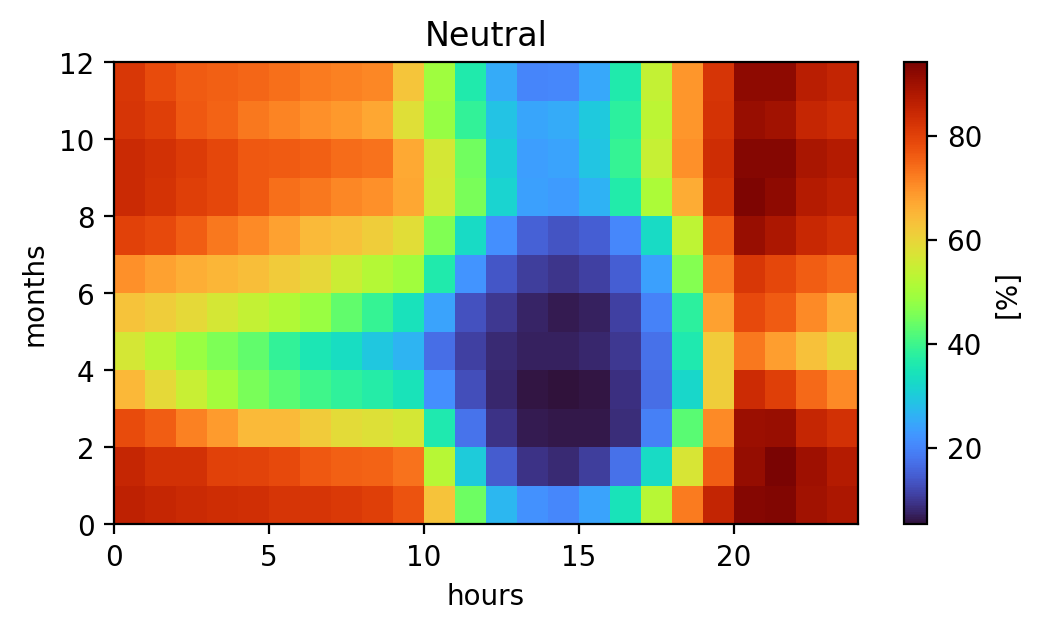
\includegraphics[width=\linewidth]{neutral_35years.png}
    \end{minipage}
    \hfill
    \begin{minipage}{0.49\textwidth}
        \centering
        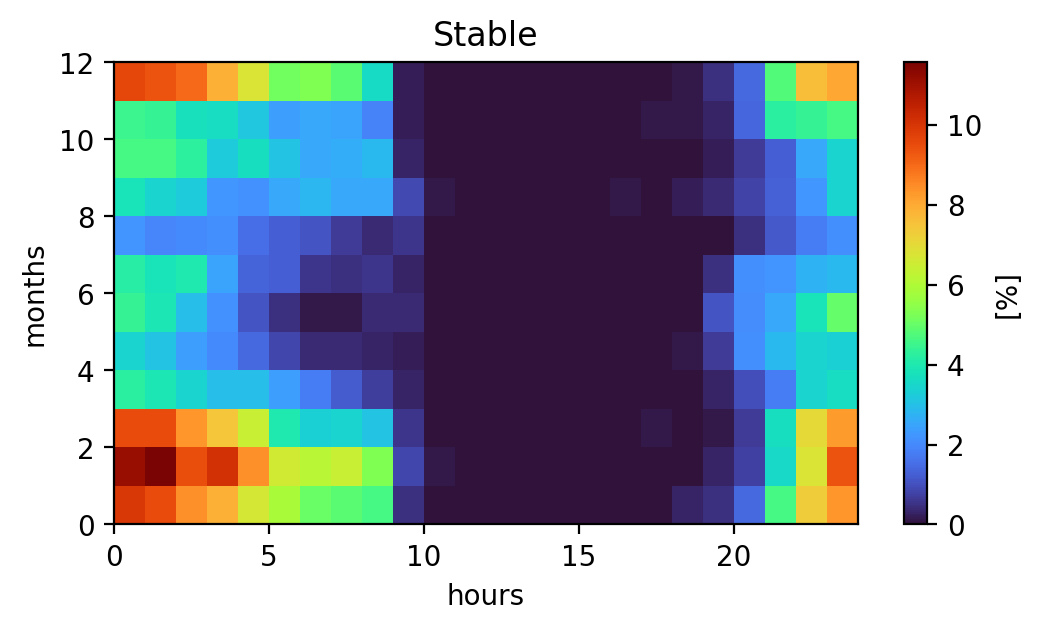
\includegraphics[width=\linewidth]{stable_35years.png}
    \end{minipage}

    \vspace{0.5cm}
    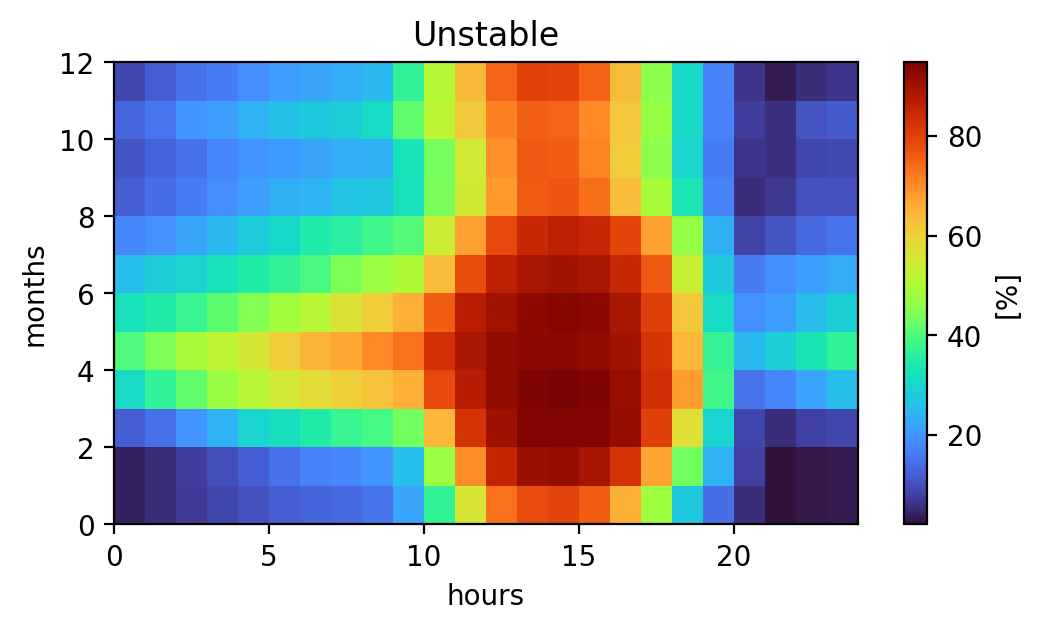
\includegraphics[width=0.49\textwidth]{unstable_35years.png}
    
    \captionof{figure}{Distribución mensual/horaria de condiciones de estabilidad atmosférica (1990-2024). Eje X: Hora del día (UTC), Eje Y: Mes.}
    \label{fig:clima}
\end{center}
%%%%
\begin{itemize}
    \item \textbf{Condiciones de Inestabilidad}: Máximos entre 10:00-18:00 UTC (Figura 1c), asociados a calentamiento solar. estacionalmente mayor cantidad de eventos entre enero y agosto.
    \item \textbf{Condiciones de Estabilidad}: Mayor frecuencia desde las 23:00 hasta las 04:00 UTC. Domina la poca frecuencia de esta condiciones principalmente entre las 09:00 y 20:00 horass durante todo el año (Figura 1b).
    \item \textbf{Condiciones Neutras}: Picos post 19:00 UTC (Figura 1a), favorecidos por enfriamiento radiativo. Mayor frecuencia desde agosto hasta febrero.
    
\end{itemize}

%% ------------------------- RELEVANCIA PARA PETROBRAS -------------------------
% Estos patrones permiten:
% \begin{itemize}
%     \item Programar mantenimiento en períodos estables/nocturnos.
%     \item Maximizar generación en horas neutras/inestables.
%     \item Evitar daños por turbulencia extrema.
% \end{itemize}

% ------------------------- REFERENCIAS -------------------------

\bibliographystyle{apalike}  % Solo aquí, sin duplicados
\bibliography{latex22}         % Nombre de tu archivo .bib
\end{document}